%%% Local Variables:
%%% TeX-command-extra-options: "-shell-escape"
%%% End:

\documentclass{beamer}

\usepackage[utf8]{inputenc}
%%%\usetheme{Madrid}
\usetheme{Berkeley}
\usecolortheme{beaver}
\usepackage{minted}
\usepackage{graphicx}
\graphicspath{{./images/}}

\usepackage{hyperref}
\hypersetup{
    colorlinks=true,
    linkcolor=blue,
    filecolor=magenta,      
    urlcolor=cyan,
}

\newminted{apache}{fontsize=\scriptsize, 
  numbersep=8pt,
  gobble=4,
  frame=lines,
  fontfamily=courier,
  fontsize=\small,
  bgcolor=bg,
  framesep=3mm} 

\newminted{docker}{fontsize=\scriptsize, 
  numbersep=8pt,
  gobble=4,
  frame=lines,
  fontfamily=courier,
  fontsize=\small,
  bgcolor=bg,
  framesep=3mm
} 

\newminted{yaml}{fontsize=\scriptsize, 
  numbersep=8pt,
  gobble=4,
  frame=lines,
  fontfamily=courier,
  fontsize=\small,
  bgcolor=bg,
  framesep=3mm} 

\newminted{bash}{fontsize=\scriptsize, 
  numbersep=8pt,
  gobble=4,
  frame=lines,
  fontfamily=courier,
  fontsize=\small,
  bgcolor=bg,
  framesep=3mm} 

% Information to be included in the title page:
\title{Openshift}
\subtitle{Introduction to the Side Car}
\author{Laurent Valeyre}
\institute{Orange}
\date{August 2018}

%%%\logo{
\includegraphics[height=0.7cm]{2753308_0.jpg}}
\logo{
\includegraphics[height=1.5cm]{orange.png}}

\begin{document}

\frame{\titlepage}

\definecolor{bg}{rgb}{0.95,0.95,0.95}

\begin{frame}
  \frametitle{Table of contents}
  \tableofcontents
\end{frame}

%%% Local Variables:
%%% TeX-command-extra-options: "-shell-escape"
%%% End:

\section{The base}

\subsection{Containers}

\begin{frame}[fragile]
  \frametitle{Containers}
\begin{figure}[ht]
  \caption{Why Containers}
  \centering
  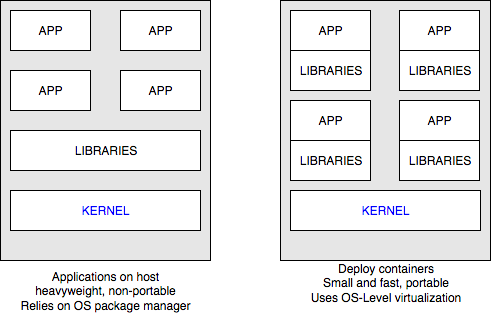
\includegraphics[scale=0.5]{ContainerDiagram.png}
  \label{fig:ContainerDiagram}
\end{figure}
\end{frame}

\subsection{Understanding Pods}

\begin{frame}
  \frametitle{Understanding Pods}
  \begin{itemize}
  \item<1->A \emph{Pod} is the smallest and simplest unit in the Kubernetes object model that we create or deploy.
  \item<2->A Pod represents a running process on our cluster.
    \begin{itemize}
    \item<3->A \emph{Pod} encapsulates an application container (or, in some cases, multiple containers)
    \item<4->A \emph{Pod} storages resources
    \item<5->A \emph{Pod} has an unique network IP
    \end{itemize}
  \item<6->A \emph{Pod} represents an unit of deployment:
  \end{itemize}
\end{frame}

\subsection{Main Ways}

\begin{frame}
  \frametitle{Main ways}
  Pods in a Kubernetes cluster can be used in two main ways:
  \begin{itemize}
  \item<2->Pods that run a single container (most common Kubernetes use case)
  \item<3->Pods that run multiple containers that need to work together(encapsulate an application composed of multiple co-located containers that tightly coupled)
  \end{itemize}
\end{frame}

\subsection{Patterns}

\begin{frame}[fragile]
  \frametitle{Patterns for Composite Containers: Sidecar}
  \begin{figure}[ht]
    \caption{schema of our Sidecar}
    \centering
    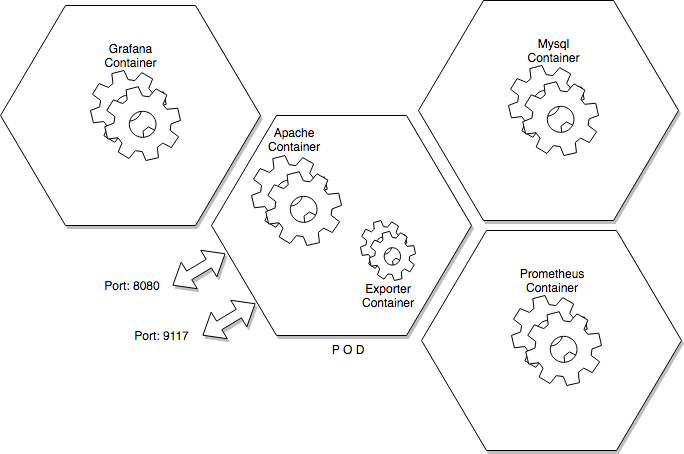
\includegraphics[scale=0.4]{SidecarDiagram.png}
    \label{fig:SidecarDiagram}
  \end{figure}
\end{frame}


%%% Local Variables:
%%% TeX-command-extra-options: "-shell-escape"
%%% End:

\section{Use case}

\subsection{Apache Status}

\begin{frame}[fragile]
  \frametitle{Apache status}
  Module to enable the output statistic of \emph{Apache}.

  \begin{figure}
    \begin{apachecode}
      <Location /server-status>
        SetHandler server-status
        Order deny,allow
        Allow from all
      </Location> ExtendedStatus On>
    \end{apachecode}
    \caption{status.conf}

    This module has to be copied in the \emph{/etc/apache2/mods-enabled/} directory.
  \end{figure}
\end{frame}

\subsection{Dockerfile}

\begin{frame}[fragile]
  \frametitle{Dockerfile}
  The \emph{Dockerfile} includes the copy of the \emph{Apache} module\\
  Important to add the switching between \textit{root} and \textit{1001} user
  \begin{figure}
    \begin{dockercode}
      FROM ubuntu:latest
      USER root
      ...
      RUN a2enmod status
      COPY status.conf /etc/apache2/mods-enabled/
      EXPOSE 8080
      USER 1001
      CMD ["/usr/sbin/apache2ctl", "-DFOREGROUND"]
    \end{dockercode}
    \caption{Dockerfile}
  \end{figure}
\end{frame}

\subsection{Secret Access}

\begin{frame}[fragile]
  \frametitle{Secret Access}
  And because the credential of \emph{GITLAB}, we'll use the login/password based on the token initialized in our profile
  \begin{figure}
    \begin{yamlcode}
      apiVersion: v1
      kind: Secret
      metadata:
        name: gitlab-secret
        namespace: cdnapi
      type: kubernetes.io/basic-auth
      data:
        username: c3Bpa2U=
        password: dmFsZW50aW5l
    \end{yamlcode}
    \caption{gitlab-secret.yaml}
  \end{figure}
\end{frame}

\subsection{The application}

\begin{frame}[fragile]
  \frametitle{New Project}
  It's time to create our new project \emph{cdnapi}, similar to a namespace
  \begin{bashcode}
    $ oc new-project cdnapi \
    --display-name='CDN API Project' \
    --description='CDN API Project'
  \end{bashcode}
\end{frame}

\begin{frame}[fragile]
  \frametitle{Secret Access}
  The \emph{username} and \emph{password} are encoded to Base64 format. Finally we load the new \emph{secret}
  \begin{bashcode}
    $ echo -n 'spike' | base64
    c3Bpa2U=
    $ echo -n 'valentine' | base64
    dmFsZW50aW5l
    $ oc create -f gitlab-secret.yaml
  \end{bashcode}
\end{frame}

\begin{frame}[fragile]
  \frametitle{New Application}
  It's time to create our application
  \begin{bashcode}
    $ oc new-app https://gitlab.forge.orange-labs.fr/\
    laov6410/cdnselect.git --name 
    $ oc set build-secret --source bc/cdnapi gitlab-secret
    $ oc expose service cdnapi
    $ oc get all name --selector app=cdnapi
  \end{bashcode}
\end{frame}

\subsection{Deployment and Service}

\begin{frame}[fragile]
  \frametitle{Item To Modify}
  2 parts will be modified to adapted to our application
  \begin{itemize}
  \item DeploymentConfig
  \item Service
  \end{itemize}
\end{frame}

\begin{frame}[fragile]
  \frametitle{DeploymentConfig}
  We edit \emph{DeploymentConfig}
  \begin{bashcode}
    $ oc edit dc/cdnapi
  \end{bashcode}
  and we add
  \begin{yamlcode}
    spec:
      containers:
      - name: apache-exporter
        image: previousnext/apache-exporter
        command: [ "apache_exporter", "-scrape_uri", \
        "http://127.0.0.1:8080/server-status/?auto" ]
        ports:
        - containerPort: 9117
  \end{yamlcode}
\end{frame}

\begin{frame}[fragile]
  \frametitle{Service}
  We edit \emph{service}
  \begin{bashcode}
    $ oc edit svc/cdnapi
  \end{bashcode}

  \begin{yamlcode}
    spec:
      ...
      - name: 9117-tcp
        port: 9117
        protocol: TCP
        targetPort: 9117
  \end{yamlcode}
  9117 is The port related to \emph{exporter apache}
\end{frame}

\begin{frame}[fragile]
  \frametitle{Finally}
  Finally we create our new application from this \emph{yaml} file
  \begin{bashcode}
    $ oc get svc --selector "app=cdnapi"
    NAME      TYPE        CLUSTER-IP      PORT(S)           
    selector  ClusterIP   172.30.127.98   8080/TCP,9117/TCP
    $ oc describe dc/cdnapi
  \end{bashcode}
  Et voila...
\end{frame}


%%%Local Variables:
%%% TeX-command-extra-options: "-shell-escape"
%%% End:


\section{Introduction}

\section{Prometheus}

\subsection{Install}

\begin{bashcode}
  $ oc new-app prom/prometheus
  $ oc expose service prometheus
\end{bashcode}

\section{Grafana}

\subsection{Install}

\begin{bashcode}
  $ oc new-app grafana/grafana
  $ oc expose service grafana
\end{bashcode}


%%% Local Variables:
%%% TeX-command-extra-options: "-shell-escape"
%%% End:

\section{Pipeline and CI}

\begin{frame}
\begin{figure}[ht]
  \caption{diagram of different projects}
  \centering
  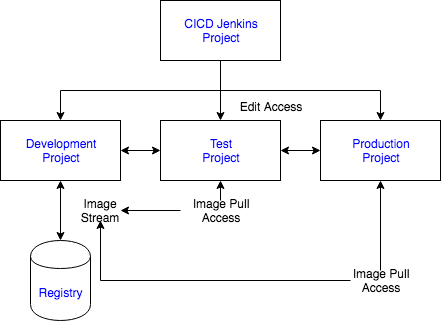
\includegraphics[scale=0.6]{ProjectPipelineDiagram.png}
  \label{fig:ProjectPipelineDiagram}
\end{figure}
\end{frame}

\begin{frame}
  \begin{itemize}
  \item Project CICD Containing our Jenkins instance
  \item Development For building and developing our application images
  \item Testing For testing our application
  \item Production Hosting our production application
  \end{itemize}
\end{frame}

\begin{frame}[fragile]
  \frametitle{Create Projects}
  \begin{bashcode}
    $ oc login -u developer -p developer
    $ oc new-project cicd --display-name='CICD Jenkins' \
    --description='CICD Jenkins'
    $ oc new-project development \
    --display-name='Development' --description='Development'
    $ oc new-project testing --display-name='Testing' \
    --description='Testing'
    $ oc new-project production --display-name='Production' \
    --description='Production'
  \end{bashcode}
\end{frame}

\begin{frame}[fragile]
  \frametitle{RBAC}
  
  \begin{bashcode}
    $ oc policy add-role-to-user edit \
    system:serviceaccount:cicd:jenkins -n development
    $ oc policy add-role-to-user edit \
    system:serviceaccount:cicd:jenkins -n testing
    $ oc policy add-role-to-user edit \
    system:serviceaccount:cicd:jenkins -n production
  \end{bashcode}
\end{frame}

\begin{frame}[fragile]
  \frametitle{RBAC}
  \begin{bashcode}
    $ oc policy add-role-to-group system:image-puller \
    system:serviceaccounts:testing -n development
    $ oc policy add-role-to-group system:image-puller \
    system:serviceaccounts:production -n development
  \end{bashcode}
\end{frame}


\subsection{Deploy Jenkins and Our Pipeline Definition}

\begin{frame}[fragile]
  \frametitle{Jenkins}
  Deploy a Jenkins ephemeral instance in \textit{cicd} project
  \begin{bashcode}
    $ oc project cicd
    $ oc new-app --template=openshift/jenkins-persistent
    $ oc status
  \end{bashcode}
  Let's create the pipeline itself.
  \begin{bashcode}
    $ oc create -n cicd -f \
    https://raw.githubusercontent.com/devops-with-openshift\
    /pipeline-configs/master/pipeline.yaml
  \end{bashcode}
\end{frame}

\subsection{Deploy Our Sample Application}
\begin{frame}[fragile]
  \frametitle{Jenkins}
  \begin{bashcode}
    $ oc project development
    $ oc create new-app --name=cdnapi \
    https://github.com/gandalf-the-white/faye.git
    $ oc expose svc/cdnapi
  \end{bashcode}
\end{frame}


\begin{frame}[fragile]
  \frametitle{Jenkins}
  \begin{bashcode}
    $ oc project testing
    $ oc create dc cdnapi \
    --image=172.30.1.1:5000/development/cdnapi:promoteQA
    $ oc rollout cancel dc/cdnapi
  \end{bashcode}
\end{frame}

\begin{frame}[fragile]
  \frametitle{Patch}
  \begin{bashcode}
    $ oc patch dc/cdnapi -p \
    '{"spec":{"template":\
        {"spec":{"containers":\
            [{"name":"default-
              container","imagePullPolicy":"Always"\
            }]}}}}'
    $ oc rollout cancel dc/cdnapi
  \end{bashcode}
\end{frame}

\begin{frame}[fragile]
  \frametitle{Expose}
  \begin{bashcode}
    $ oc expose dc cdnapi --port=8080
    $ oc expose svc/cdnapi
  \end{bashcode}
\end{frame}

\begin{frame}[fragile]
  \frametitle{Jenkins}
  \begin{bashcode}
    $ oc project production
    $ oc create dc cdnapi \
    --image=172.30.1.1:5000/development/cdnapi:promotePRD
    $ oc rollout cancel dc/cdnapi
  \end{bashcode}
\end{frame}

\begin{frame}[fragile]
  \frametitle{Patch}
  \begin{bashcode}
    $ oc patch dc/cdnapi -p \
    '{"spec":{"template":\
        {"spec":{"containers":\
            [{"name":"default-
              container","imagePullPolicy":"Always"\
            }]}}}}'
    $ oc rollout cancel dc/cdnapi
  \end{bashcode}
\end{frame}

\begin{frame}[fragile]
  \frametitle{Expose}
  \begin{bashcode}
    $ oc expose dc cdnapi --port=8080
    $ oc expose svc/cdnapi
  \end{bashcode}
\end{frame}

%%% Local Variables:
%%% TeX-command-extra-options: "-shell-escape"
%%% End:

\section{Links}

\begin{frame}
  \frametitle{links}
  \url{https://kubernetes.io/blog/2015/06/the-distributed-system-toolkit-patterns/}
  \url{https://www.robustperception.io/openshift-and-prometheus}
  \url{http://widerin.net/blog/official-grafana-docker-image-on-openshift/}
\end{frame}

\end{document}
